Bien que les étapes de traitement automatiques implémentées au dessus du
module de base aient une cohérence logique, dans les faits le seul
principe obligatoire est la présence de l'entité de base (la région
d'image) sur laquelle effectuer l'action. Ensuite, les traitements ne
suivent pas obligatoirement une séquence chronologique stricte. La
première étape de sélection de zones d'images d'intérêt (automatique ou
manuelle) peut être seule considérée comme nécessaire et suffisante pour
démarrer une analyse approfondie des sources. La refonte des processus
prend donc en compte la possibilité de procéder dans un ordre aléatoire.

\hypertarget{modules-optionnels}{%
\subsection{Modules optionnels}\label{modules-optionnels}}

Le \textit{workflow} commence par l'enregistrement d'un document (\wit ou
\ser) avec ses métadonnées, et l'import d'une numérisation associée. Il
est alors visualisable.

L'application contient des modules optionnels à activer ou désactiver
selon les besoins. Les modules d'ores et déjà proposés utilisent la
\cv, ils sont aujourd'hui au nombre de trois~:
l'extraction, la recherche de similarité et la vectorisation. Les outils
de \dl sont mis à disposition via une \api accueillant
les modèles pour l'inférence et séparée de l'application permettant la
gestion des données, le lancement des traitements, la visualisation et
la correction des résultats.

L'extraction automatique détecte les zones d'intérêt dans les
numérisations et les indexe dans le système \sas. La tâche se déclenchait
initialement systématiquement lors de l'enregistrement du témoin dans la
base de données (la méthode de classe qui permettait l'enregistrement du
\wit lançait un \emph{thread} en même temps). Pour plus de souplesse
dans les processus, l'annotation automatique -- en tant que module
optionnel -- est aujourd'hui déclenchée par une action de l'utilisateur.rice,
via le formulaire de lancement de traitement. Si le chercheur.se fait le
choix d'appliquer une extraction automatique sur sa/ses sources, une
requête \api lance l'inférence avec les scripts de \yolov sur le \gpu
Dishas-ia, et déclenche l'annotation automatique de diagrammes dans les
scans numérisés. À l'issue de ce processus, l'\api génère un fichier
texte structuré, contenant pour chaque image son identifiant unique et
les coordonnées précises des régions détectées comme étant des
diagrammes. Ces informations sont ensuite renvoyées à l'application, le
fichier est enregistré et les informations qu'il contient sont indexées
sous forme d'annotations dans le \man \iiif correspondant à chaque
numérisation.

La présence de ces régions découpées au sein des images numérisées
constitue une condition préalable indispensable à l'exécution de
traitements ultérieurs.

Le principe du traitement groupé normalise le processus de lancement des
tâches et le formatage des données à envoyer à l'\api. Un fichier \json,
vecteur de la communication entre les deux composants, structure une
liste d'\URLs \iiif, chacune pointant vers une image ou une région d'image
d'intérêt, ainsi que des métadonnées
descriptives.

Le \json est formaté par une fonction appelée \texttt{prepare\_request}, et
qui existe pour tous les modules, ci-dessous, par exemple, pour l'extraction~:

\begin{lstlisting}[language=python, frame=single, breaklines=true, caption={Fonction \texttt{prepare\_request du module d'extraction}}]
#vhs/app/regions/utils.py
def prepare_request(witnesses, treatment_id):
    manifests = {}

    try:
        for witness in witnesses:
            if witness.has_regions():
                log(
                    f"[regions_request] Witness {witness.get_ref()} already has regions"
                )
                pass
            else:
                digits = witness.get_digits()
                for digit in digits:
                    manifests.update({witness.get_ref(): digit.gen_manifest_url()})

        if manifests:
            return {
                "experiment_id": f"{treatment_id}",
                "documents": manifests,
                "model": f"{EXTRACTOR_MODEL}",  # Use only if specific model is desire
                "callback": f"{APP_URL}/{APP_NAME}/get-regions",  # URL to which the regions file must be sent back
                "tracking_url": f"{APP_URL}/{APP_NAME}/api-progress",
            }
        else:
            return {
                "message": f"Regions were already extracted for all the selected {WIT}es"
                if APP_LANG == "en"
                else f"Les régions ont déjà été extraites pour tous les {WIT}s sélectionnés"
            }

    except Exception as e:
        log(
            f"[prepare_request] Failed to prepare data for regions request",
            e,
        )
        raise Exception(f"[prepare_request] Failed to prepare data for regions request")
\end{lstlisting}

La fonction reçoit une liste de \wits générée par une tâche
appelée par la méthode \texttt{treatment\_post\_save} de l'entité \tr~:

\begin{lstlisting}[language=python, frame=single, breaklines=true, caption={Création d'une tâche à la création d'un \tr.}]
# vhs/app/webapp/models/treatment.py
@receiver(post_save, sender=Treatment)
def treatment_post_save(sender, instance, created, **kwargs):
    if created:
        get_all_witnesses.delay(instance)
\end{lstlisting}

\begin{lstlisting}[language=python, frame=single, breaklines=true, caption={Tâche qui rassemble les \wits et lance l'action sur les documents.}]
# vhs/app/webapp/tasks.py
@celery_app.task
def get_all_witnesses(treatment):
    try:
        witnesses = treatment.get_witnesses()
        treatment.start_task(witnesses)
    except Exception as e:
        treatment.on_task_error(
            {
                "error": f"Error when retrieving documents from set: {e}",
                "notify": treatment.notify_email,
            },
        )
\end{lstlisting}

Ce formatage normalisé permet d'adapter tout le processus de lancement
à une variété de tâches. L'envoi d'une requête \http à l'\textit{endpoint} d'\api
appropriée déclenche l'exécution du traitement. Une fois l'inférence
terminée, les résultats sont retournés à l'application et une
notification est envoyée à l'utilisateur.rice. L'instance \tr sert
aussi à standardiser le suivi en temps réel de l'état d'avancement de
chaque tâche (Fig. \ref{fig:treatment}).

\begin{figure}[H]
          \begin{center}
          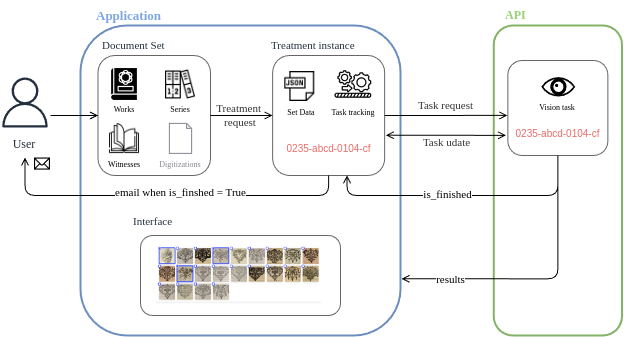
\includegraphics[height=8cm]{figues/treatment.png}
          \end{center}
          \caption{Fonctionnement de l'envoi d'un traitement à l'\api.*\protect\footnotemark}
          \label{fig:treatment} \end{figure}

\footnotetext{Les schémas suivis d'un astérisque sont prélevés ou inspirés de la documentation technique interne créée par les développeur.ses du projet \eida et de l'\iscd.}

Le système est ainsi conçu pour être évolutif. Les utilisateur.rices peuvent
envisager d'étendre ses capacités en y intégrant de nouveaux modules.
Parmi les fonctionnalités potentielles, on peut citer~: des outils
d'édition des diagrammes (ce qui intéresse spécifiquement \eida), des
algorithmes de classification et de \textit{clustering}, un modèle de
reconnaissance de filigranes, ou encore l'intégration d'une \textit{pipeline} de
transcription de textes comme e-Scriptorium.

La conception modulaire du système permet de configurer des \textit{pipelines} de
traitement personnalisés. Chaque module peut être activé ou désactivé
indépendamment des autres. Les traitements peuvent être combinés selon
les besoins spécifiques. Par exemple, le calcul de similarité et la
vectorisation peuvent être réalisés parallèlement, et sans passer par
une étape d'extraction automatique préalable, si les documents ont été
annotés manuellement.

\hypertarget{module-similarite-workflow-detaille}{%
\subsubsection{\texorpdfstring{Module \emph{Similarité}~: workflow
détaillé}{Module Similarité~: workflow détaillé}}\label{module-similarite-workflow-detaille}}

Le module \textit{similarity retrieval} inclut le calcul de scores de
similarité selon différentes méthodes (\textit{cosine distance}, Segswap, etc.)\footnote{Voir le \hyperlink{similarite}{chapitre IV, 2.2}} et la catégorisation de ces similarités (\textit{exact match},
\textit{partial}, \textit{personnal}, etc.)\footnote{Voir le \hyperlink{chapitre-8-interfaces}{chapitre suivant}.}. La
recherche de similarité ne fonctionne que sur les images de diagrammes
déjà extraites, identifiées grâce à des \URLs et accessibles grâce à l'\api
Image de \iiif. La tâche est lancée sur un ensemble de témoins. Pour
chaque document sélectionné, le \gpu reçoit une liste d'\URLs \iiif
pointant vers des régions d'intérêt. Les images correspondantes sont
téléchargées et des descripteurs visuels (\emph{features}) sont extraits
grâce au réseau de neurones. L'attribution d'un indice de similarité se
fait par la comparaison de plusieurs métriques des vecteurs de
descripteurs. Les résultats sont stockés dans un fichier NumPy. Ce
fichier, qui contient les scores de similarité pour toutes les paires
d'images comparées, est retourné à l'application.

L'interface utilisateur.rice permet une exploration interactive de ces
résultats. Pour une image donnée, il est possible de visualiser
dynamiquement les images les plus similaires provenant d'autres
documents. Cette fonctionnalité repose sur l'agrégation des scores de
similarité au niveau de chaque image.

\hypertarget{module-vectorisation-workflow-detaille}{%
\subsubsection{\texorpdfstring{Module \emph{Vectorisation}~: workflow
détaillé}{Module Vectorisation~: workflow détaillé}}\label{module-vectorisation-workflow-detaille}}

La tâche de vectorisation consiste en la génération de fichiers \svgs à
partir des images extraites. Tout comme la recherche de similarité,
cette opération s'applique à des régions d'images préalablement
indexées. La vectorisation peut être intégrée à différents points du
\textit{pipeline} de traitement~; elle peut être exécutée avant ou après la
recherche de similarité, en fonction des besoins.

Comme pour la similarité, une liste d'\URL structurées dans un fichier
\json est envoyée par une requête \http POST~: sa réception lance la
chaîne de traitement dans l'\api, qui télécharge les images à partir
des \URLs spécifiées dans le fichier \json. Les \svgs résultants de
l'inférence avec le modèle sont compressés dans un fichier \textsc{zip}. Le
fichier \textsc{zip} contenant les \svgs est renvoyé à l'application via une
requête \http POST. Enfin, l'application enregistre le fichier \textsc{zip} sur le
serveur, rendant ainsi les \svg accessibles à l'utilisateur.rice.

L'inférence du modèle de vision nécessite des ressources
computationnelles importantes. L'implémentation dans l'\api doit prendre
en compte ces exigences de performance et garantir en conséquence une
scalabilité adéquate. Pour éviter la surcharge et gérer les multiples
requêtes sur le \gpu, l'\api utilise un système de \textit{threading}. Ce système,
nommé Dramatiq, gère les tâches de fond et traite les requêtes entrantes
en imposant leur traitement séquentiel. Dramatiq fonctionne avec Redis,
un magasin de valeurs-clés, servant de base de données intermédiaire qui
assigne les tâches aux \emph{workers}. Dramatiq gère la bonne tenue des
tâches, faisant l'intermédiaire entre les \textit{workers} et le système de
\textit{login}. De la même manière, pour la réception ou l'envoi de données
volumineuses, l'application emploie Celery, un système de \textit{threading}
similaire.

\begin{figure}[H]
          \begin{center}
          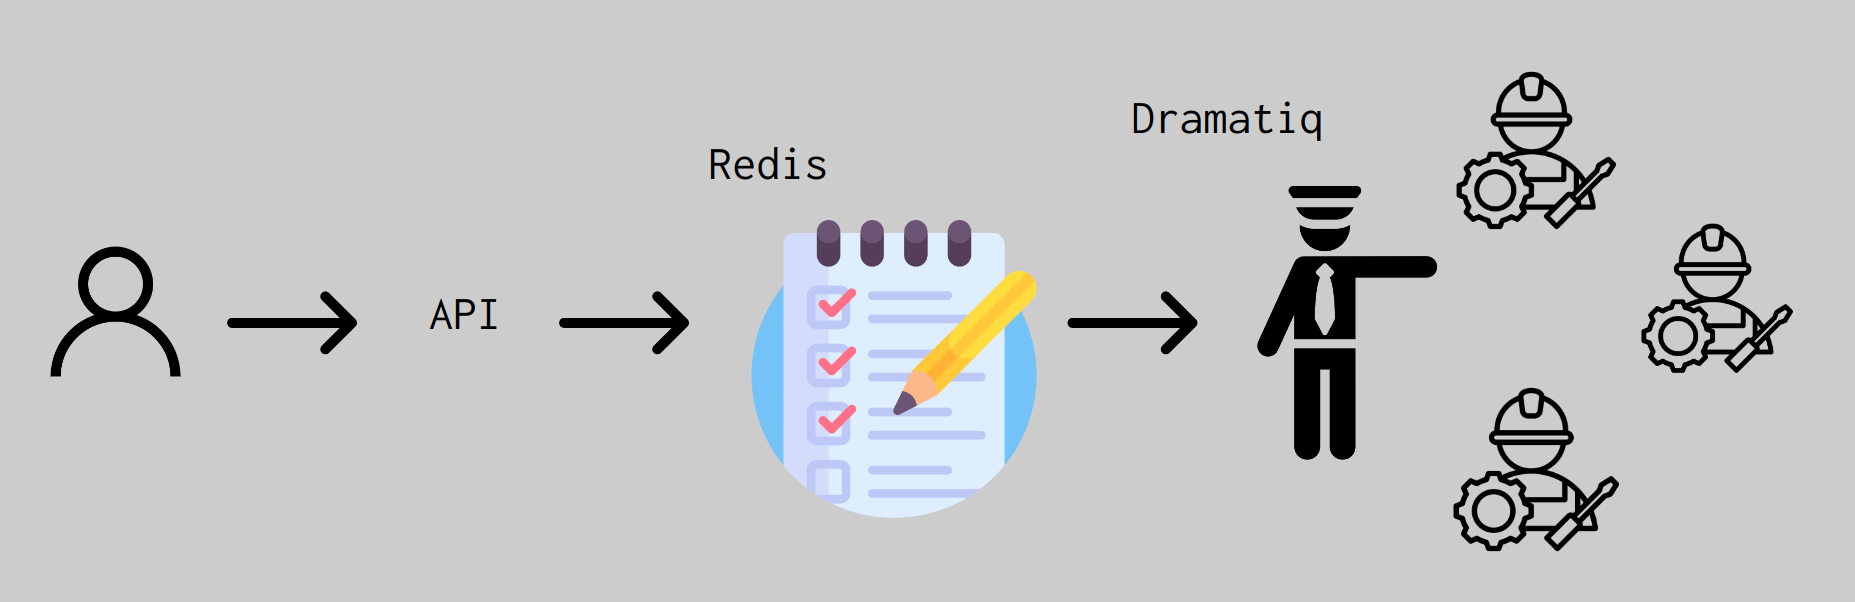
\includegraphics[height=4cm]{figues/dramatiq.png}
          \end{center}
          \caption{Fonctionnement du système de \textit{threading} de l'\api.}
          \label{fig:dramatiq} \end{figure}

Le cœur de ce système modulaire réside dans le développement de trois
interfaces principales qui guideront le chercheur.se dans les processus~:
la recherche d'entités, leur sélection dans un panier et le
déclenchement des traitements.

\hypertarget{alternance-detapes-automatiques-et-detapes-manuelles}{%
\subsection{Alternance d'étapes automatiques et d'étapes
manuelles}\label{alternance-detapes-automatiques-et-detapes-manuelles}}

Prenant en compte les biais potentiels des traitement d'\ia,
l'implémentation des tâches de vision doit être pensée de manière à
autoriser la correction de l'inférence des modèles, d'une part pour
avoir des résultats finaux plus pertinents, et d'autre part pour
produire des données annotées dédiés au \emph{fine-tuning} des modèles.

En effet~:

\begin{kwote}
``Data analysis for Art History means the introduction of quantitative
methods into a field that has used exclusively qualitative methods
throughout its existence. However, these quantitative methods are not a
substitute for conventional methods, but an addition. Results of data
analysis can help to answer to our research questions, but may also
spark new hypotheses that can be followed using a bouquet of methods
that Art History has. For some, Big Data seems to be the end of theory
but one could also argue that Data Analytics helps us to see the big
picture and create new hypotheses for qualitative research. This way,
the computer remains a tool in the hands of the researcher, or as Steve
Jobs defined the role of the computer to the human,''a bicycle for the
mind''.\footcite[p.28]{klinke_big_2016}
\end{kwote}

Les méthodes quantitatives sur la donnée de masse sont une étape
préliminaire à la recherche qualitative. Les résultats nécessitent
toujours une interprétation~; ils ne remplacent pas les hypothèses, mais
en sont la prémisse.

\begin{kwote}
``L'automatisation n'exclut pas un certain nombre d'actions manuelles
sur les sources, et l'utilisation d'algorithmes de vision artificielle
ne remplace pas le regard critique que peuvent porter les chercheur.ses sur
les sources~: il est donc nécessaire, dans les chaînes de traitement
définies par les projets, de trouver un équilibre entre étapes
automatiques et étapes manuelles de traitement des sources historiques,
pour assurer, en finalité, des résultats les plus pertinents
possibles.''\footcite[p.70]{norindr_traitement_2023}
\end{kwote}

\begin{kwote}
``Face à ce constat, il est nécessaire, pour les ingénieurs, de
concevoir une chaîne de traitement qui va au-delà des étapes
automatisées, et qui prend en compte la nécessité d'interventions
manuelles entre chaque traitement pour un ajustement des résultats et
une analyse primaire des données de sortie. Pour espérer produire des
recherches aux résultats pertinents, il est ainsi nécessaire de savoir
intégrer l'outil qu'est le \dl à un \textit{workflow}, et de trouver
l'équilibre entre automatisation et tâches manuelles.''\footcite[p.70]{norindr_traitement_2023}
\end{kwote}

L'\ia est employée comme un outil de
pré-traitement des sources, permettant de naviguer dans un corpus
volumineux, de créer des rapprochement pour identifier les phénomènes de
copie et d'emprunts, et/ou d'éditer les sources dans un format
sémantiquement riche qu'est le \svg. Ces traitements permettent aux
chercheur.ses de gagner un temps significatif comparé à une analyse et une
transcription manuelle des documents. L'établissement de la chaîne de
traitement se doit néanmoins de prendre en compte les limites de la
\cv. Le \textit{workflow} doit comporter suffisamment d'étapes de
correction manuelle, qui restent moins chronophages qu'une recherche et
édition manuelle des illustrations dans chaque source étudiée, et
n'en sont que d'autant plus nécessaires pour assurer la pertinence des
analyses.

Pour optimiser les performances de l'algorithme de détection, il est
nécessaire d'exclure ou d'inclure certains cas limites lors de
l'entraînement du modèle\footnote{Voir le \hyperlink{loeil-de-la-machine-avantages-et-limites}{chapitre 5, 2.3}}. Le
modèle de détection final peut alors manquer des diagrammes pertinents
pour les chercheur.ses ou, à l'inverse, détecter des illustrations sans
rapport avec leur objet d'étude.

De même, l'algorithme de similarité présente ses propres limites\footnote{Voir le \hyperlink{developpement-dune-interface-commune}{chapitre 1, 3.2}}. Les chercheur.ses ont besoin de poser un regard expert sur leurs corpus, et d'effectuer manuellement les rapprochements entre les images, ou bien de qualifier avec une plus grande finesse le type de similarité existant
entre deux images

Une étape de vérification manuelle permet donc de corriger les défauts
des modèle, notamment sa tendance à la binarité qui ne correspond pas à
la complexité du réel. Il est alors nécessaire de travailler des
interfaces de visualisation et de correction des résultats, et de
modéliser ces processus de vérification dans le \textit{workflow}. Les données
récupérées sont donc inspectées par l'œil critique du chercheur.se. La
réduction de l'automatisation au profit d'une intervention humaine
contrôlée favorise une meilleure adéquation aux besoins spécifiques de
chaque projet de recherche, bien que les chercheur.ses bénéficient la
rapidité de traitement de l'intelligence artificielle pour le traitement
de corpus volumineux. Cette approche hybride, combinant l'efficacité de
l'apprentissage profond et la précision de l'expertise humaine, optimise
ainsi la qualité globale des résultats.

La table \texttt{Regions} intègre un attribut booléen \texttt{is\_validated} indiquant si
les annotations automatiques associées à une numérisation ont été
approuvées par un chercheur.se. Pareillement, afin d'évaluer la pertinence
des scores attribués par l'algorithme de recherche de similarité, une
catégorie est associée à chaque paire d'images, permettant ainsi d'évaluer la ressemblance de ces paires selon une nomenclature
prédéfinie. Cette catégorisation, établie par les chercheur.ses, sert donc
à évaluer la qualité des scores de similarité attribués par le modèle et
constitue une métadonnée précieuse pour une utilisation personnalisée ou
pour l'amélioration du modèle. Pour pallier aux manquements de
l'algorithme, les utilisateur.rices peuvent aussi créer
manuellement des paires d'images (attribut \texttt{is\_manual} de la table
\texttt{Regions\_Pair}). De même, les \svgs ramenés en sortie du modèle de
vectorisation devront faire l'objet d'une correction manuelle, dans une
interface dédiée, par les chercheur.ses, avant d'envisager leur
exploitation.

Ainsi, pour que les avantages de la \cv soient
pleinement exploités, il est important de disposer d'interfaces
utilisateur.rice interactives pour la visualisation et la correction des
résultats, facilitant leur compréhension et permettant de tester
différentes hypothèses (Fig. \ref{fig:workflow}).

 \begin{figure}[H]
          \begin{center}
          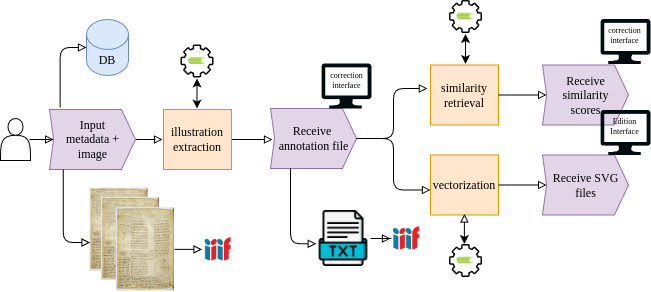
\includegraphics[height=6cm]{figues/workflow.png}
          \end{center}
          \caption{\emph{Workflow} schématique.*}
          \label{fig:workflow} \end{figure}

Pour conclure, l'application, conçue selon une architecture modulaire,
s'adresse aussi bien aux utilisateur.rices recherchant des fonctionnalités de
base qu'aux équipes de recherche souhaitant personnaliser leur
environnement de travail. En offrant un ensemble de modules génériques,
le projet \aikon fournit un point de départ solide pour des projets plus
ambitieux. Les équipes d'ingénieurs peuvent ainsi se concentrer sur le
développement de modules spécifiques répondant à leurs besoins précis,
sans avoir à reconstruire l'ensemble de la plateforme. Cette approche
favorise l'innovation et permet de créer des solutions sur mesure en
réduisant le coût de développement.
